\section{Выпуклые оболочки, алгоритма Джарвиса, Грэхема и QuickHull.}

\begin{definition}
	\textbf{Выпуклое множество} --- такое множество точек, что, для любых двух точек множества, все точки на отрезке между ними тоже принадлежат этому множеству.
\end{definition}

\begin{definition}
	\textbf{Выпуклая оболочка множества точек} --- такое выпуклое множество точек, что все точки фигуры также лежат в нем.
\end{definition}

\begin{definition}
	\textbf{Минимальная выпуклая оболочка множества точек} --- это минимальная по площади выпуклая оболочка.
\end{definition}

\subsection*{Алгоритмы построения выпуклой оболочки}

\subsection{Алгоритм Джарвиса}
По-другому "Gift wrapping algorithm" (Заворачивание подарка). Он заключается в том, что мы ищем выпуклую оболочку последовательно, против часовой стрелки, начиная с определенной точки.

\textbf{Описание алгоритма}

\begin{enumerate}
	\item Возьмем точку $p_0$ нашего множества с самой маленькой $у$ координатой (если таких несколько, берем самую правую из них). 
	Добавляем ее в ответ.
	\item На каждом следующем шаге для последнего добавленного pi
	ищем $p_i+1$ среди всех недобавленных точек и $p_0$
	с максимальным полярным углом относительно $p_i$ (Если углы равны, надо сравнивать по расстоянию). Добавляем pi+1 в ответ. 
	Если $p_i+1==p_0$, заканчиваем алгоритм
\end{enumerate}

\begin{figure}[h!]
	\centering
	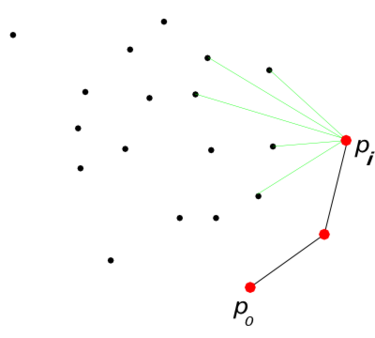
\includegraphics[width=0.4\linewidth]{img_easy/13_1.png}
	\captionsetup{labelformat=empty}
	\caption{Промежуточный шаг алгоритма. 
		Для точки $p_i$ ищем следующую перебором.}
\end{figure}
\textbf{Корректность}
Точка $p_0$, очевидно, принадлежит оболочке. На каждом последующем шаге алгоритма мы получаем прямую $p_{i-1}pi$, по построению которой все точки множества лежат слева от нее. 
Значит, выпуклая оболочка состоит из $p_i$-х и только из них.

\textbf{Сложность}

Добавление каждой точки в ответ занимает $O(n)$ времени, всего точек будет $k$, поэтому итоговая сложность $O(nk)$. В худшем случае, когда оболочка состоит из всех точек сложность $O(n^2)$.

\subsection{Алгоритм Грэхема}
Алгоритм заключается в том, что мы ищем точки оболочки последовательно, используя стек.

\textbf{Описание алгоритма}

\begin{enumerate}
	\item Находим точку $p_0$
	нашего множества с самой маленькой у-координатой (если таких несколько, берем самую правую из них), добавляем в ответ.
	\item Сортируем все остальные точки по полярному углу относительно $p_0$.
	\item Добавляем в ответ $p_1$ --- самую первую из отсортированных точек.
	\item Берем следующую по счету точку t.
	Пока t и две последних точки в текущей оболочке $p_i$ и $p_i-1$ образуют неправый поворот (вектора $p_it$ и $p_{i-1}p_i$), удаляем из оболочки $p_i$.
	\item Добавляем в оболочку $t$.
	\item Делаем п.4, пока не закончатся точки
\end{enumerate}

\subsection*{Корректность}

Докажем, что на каждом шаге множество $P_i$-тых является выпуклой оболочкой всех уже рассмотренных точек. Доказательство проведем по индукции.

\begin{itemize}
	\item \textbf{База.} Для трёх первых точек утверждение, очевидно, выполняется.
	\item \textbf{Переход.} Пусть для $i-1$ точек оболочки совпадают. Докажем, что и для $i$ точек они совпадут.
\end{itemize}

Рассмотрим истинную оболочку $ch(S \cup i) = ch(S) \cup i \setminus P$, где $P$ --- множество всех точек из $ch(S)$, видимых из $i$. Так как мы добавляли точки в нашу оболочку против часовой стрелки и так как $i$-тая точка лежит в $ch(S \cup i)$, то $P$ состоит из нескольких подряд идущих последних добавленных в оболочку точек, и именно их мы удаляем на текущем шаге. Поэтому наша оболочка и истинная для $i$ точек совпадают.

Тогда по индукции оболочки совпадают и для $i = n$.

\subsection*{Сложность}

Сортировка точек занимает $O(n \log n)$ времени. При обходе каждая точка добавляется в ответ не более одного раза, поэтому сложность этой части --- $O(n)$. Суммарное время --- $O(n \log n)$.

\subsection{Алгоритм QuickHull}

Попытаемся применить к этой задаче подход <<Разделяй и властвуй>>

\subsection*{Описание Алгоритма}

\begin{enumerate}
	\item Найдем самую левую точку $p_0$ и самую правую точку $p_1$ (Если таких несколько, выберем среди таких нижнюю и верхнюю соответственно).
	\item Возьмем все точки выше прямой $p_0 p_1$.
	\item Найдем среди этого множества точку $p_i$, наиболее отдаленную от прямой (если таких несколько, взять самую правую).
	\item Рекурсивно повторить шаги 2-3 для прямых $p_0 p_i$ и $p_i p_1$, пока есть точки.
	\item Добавить в ответ точки $p_0 \dots p_i \dots p_1$, полученные в п. 3.
	\item Повторить пункты 2-5 для $p_1 p_0$ (то есть для "нижней" половины).
	\item Ответ - объединение списков из п. 5 для верхней и нижней половины.
\end{enumerate}

\subsection*{Сложность}

Пусть время, необходимое для нахождения оболочки над некой прямой и множеством точек $S$ есть $T(S)$. Тогда
$T(S) = O(\|S\|) + T(A \in S) + T(B \in S)$, где $A, B$ --- множества над полученными прямыми. Отсюда видно, что в худшем случае, алгоритм тратит $O(n^2)$. На случайных же данных это число равно $O(n \log n)$.
